\documentclass[a4paper, 10pt]{article}

%\usepackage{scalefnt}
%\usepackage{parcolumns}

\usepackage{newclude}
% Zum Einbinden in die Zusammenfassungs-files

\usepackage{amsmath,amsthm,amsfonts,amssymb} % Verbesserter Mathesatz
\usepackage{algorithm2e}
\usepackage{bigfoot} % komplexe Fußnotenapparate(Fußnoten in Fußnoten und andere Späße)%
\usepackage{colortbl}
\usepackage[T1]{fontenc} % normaler erweitere Zeichnesatz
\usepackage{framed, color}  % Ramenpaket für zum Einfügen von schönen Ramen
\usepackage{graphicx}
\usepackage{hyperref} %used for link to creative commons license
\usepackage{listings} %for code-listings (inkl. Tab-Styling)
\usepackage{marvosym}
\usepackage{marginnote}
\usepackage{microtype} % div. Verbesserungen des Schriftsatzes (Grauwert, opt. Randausgleich, Zeilenumbruch)
%\usepackage{multirow}
\usepackage{multicol} %use this with next line for vertical divided environment
%\setlength\columnseprule{.4pt}:465
\usepackage[ngerman]{babel} % Neue Rechtschreibung
\usepackage{pifont}
\usepackage[sans]{dsfont} %für alternative Mengensymbole
\usepackage{stmaryrd} %u.a. für \lightning
\usepackage{tikz} % für Diagramme(Dia!) und Bilder (z.B. *.eps)/für ER-Diagramme/für UML-Diagramme
%\usepackage{tikz-er2} %  er-diagramme
\usepackage{tikz-uml} % uml-Diagramme
\usepackage{units} % z.B. fuer \nicefrac{}{}
\usepackage[utf8]{inputenc} % utf8 für den Editor
\usepackage{wasysym} %u.a. für \lightning
\usepackage{xcolor}


\usetikzlibrary{shapes,decorations,arrows,fit,backgrounds} %Zum diversen zeichen%
%\usetikzlibrary{automata} % für den CFlipper, wenn es den soweit ist			%
\usetikzlibrary{positioning} % positionierung
%\usetikzlibrary{shadows} % fuer schoene schlagschatten
\usetikzlibrary{automata} % für Automaten

%%%%%%%%%%%%%%%%%%%%%%%%%%%
%  Formatierung der Seite
%%%%%%%%%%%%%%%%%%%%%%%%%%%
\usepackage{fancyhdr}
\pagestyle{fancy}		% für den footer										%
\renewcommand{\headrulewidth}{0pt} % damit oben kein dummer Strich kommt		%
\fancyhead{}
\topmargin -2cm 		% Oberer Rand											%
\textheight 25cm		% Texthöhe												%
\textwidth 16.0 cm		% Textbreite											%
\oddsidemargin -0.1cm 	% Warum?												%
\newcommand{\Gruppe}[2]
{
	\lfoot{#1}
	\rfoot{#2}
}
\colorlet{shadecolor}{gray!25} % Farbe für graue Box definieren
%%%%%%%%%%%%%%%%%%%%%%%%%%%%%%%%%%%%%%%%%%%%%%%%%%%%%%%%%%%%%%%%%%%%%%%%%%%%%%%%%
%Farben die definiert werden zum schreiben und zeichnen							%
%%%%%%%%%%%%%%%%%%%%%%%%%%%%%%%%%%%%%%%%%%%%%%%%%%%%%%%%%%%%%%%%%%%%%%%%%%%%%%%%%
\xdefinecolor{schwarz}{HTML}{000000}
\xdefinecolor{dunkelGruen}{HTML}{007D00}
\xdefinecolor{dunkelBlau}{HTML}{0000A0}
\xdefinecolor{dunkelRot}{HTML}{A00000}
\xdefinecolor{dunkelGelb}{HTML}{FFAA00}
\xdefinecolor{hellesGelb}{HTML}{FFCC00}
\colorlet{dGreen}{dunkelGruen}
\colorlet{dBlue}{dunkelBlau}
\colorlet{dRed}{dunkelRot}
\colorlet{dYellow}{dunkelGelb}

%%%%%%%%%%%%%%%%%%%%%%%%%%%%%%%%%%%%%%%%%%%%%%%%%%
%Farbliche Ausgaben:
%Parameter #1: Text oder Mathematische formel...
%z.B. : \gruen{Hallo Welt Test!}
%%%%%%%%%%%%%%%%%%%%%%%%%%%%%%%%%%%%%%%%%%%%%%%%%%

\newcommand{\yellow}[1]{\textcolor{dYellow}{#1}}
\newcommand{\gray}[1]{\textcolor{gray}{#1}}
\newcommand{\red}[1]{\textcolor{red}{#1}}
\newcommand{\green}[1]{\textcolor{green}{#1}}
\newcommand{\blue}[1]{\textcolor{blue}{#1}}
\newcommand{\dGreen}[1]{\textcolor{dGreen}{#1}}
\newcommand{\dBlue}[1]{\textcolor{dBlue}{#1}}
\newcommand{\dRed}[1]{\textcolor{dRed}{#1}}

%%%%%%%%%%%%%%%%%%%%%%%%%%%%%%%%%%%%%%%%%%%%%%%%
%Konfiguration für das darstellen von Quelltext
%%%%%%%%%%%%%%%%%%%%%%%%%%%%%%%%%%%%%%%%%%%%%%%%
\lstset
{
	language=Java, % oder C++, Pascal, {[77]Fortran}, ...
	numbers=left, % Position der Zeilennummerierung
	firstnumber=auto, % Erste Zeilennummer
	basicstyle=\ttfamily, % Textgröße des Standardtexts
	keywordstyle=\ttfamily\color{dRot}, % Formattierung Schlüsselwörter
	commentstyle=\ttfamily\color{dGruen}, % Formattierung Kommentar
	stringstyle=\ttfamily\color{dBlau}, % Formattierung Strings
	numberstyle=\tiny, % Textgröße der Zeilennummern
	stepnumber=1, % Angezeigte Zeilennummern
	numbersep=5pt, % Abstand zw. Zeilennummern und Code
	aboveskip=15pt, % Abstand oberhalb des Codes
	belowskip=11pt, % Abstand unterhalb des Codes
	captionpos=b, % Position der Überschrift
	xleftmargin=10pt, % Linke Einrückung
	frame=single, % Rahmentyp
	breaklines=true, % Umbruch langer Zeilen
	showstringspaces=false, % Spezielles Zeichen für Leerzeichen
	tabsize=2,
	texcl=true
}

%%%%%%%%
% Kopf
%%%%%%%%
\newcommand{\Header}[3]
{
	{\footnotesize \parindent0em
		{\sc Universität Konstanz}                \hfill #1 \\
		{\sc Fachbereich Informatik \& Informationswissenschaft} \hfill #2 \\
		#3 \hfill \today
	}
}

%%%%%%%%%%%%%%%%%%%%%%%
% load some java code
% \loadJava{file}
%%%%%%%%%%%%%%%%%%%%%%%
\newcommand{\loadJava}[1]
{
	\lstinputlisting[language=Java]{#1.java}
}

%%%%%%%%%%%%%%%%%%%%%%%
% load some cpp code
% \loadCpp{file.cpp}
%%%%%%%%%%%%%%%%%%%%%%%
\newcommand{\loadCpp}[1]
{
	\lstinputlisting[language=C++]{#1}
}

%%%%%%%%%%%%%%%%%%%%%%%%%%%%%
% load some code
% \loadCode{Python}{file.py}
%%%%%%%%%%%%%%%%%%%%%%%%%%%%%
\newcommand{\loadCode}[2]
{
	\lstinputlisting[language=#1]{#2}
}

%%%%%%%%%%%%%%%%%%%%%%%%%%%%%%%%%%%%%%%%%%%%%%%%%%%%%%%%%%%%%%%%%%%%%%%
% some symbols
%%%%%%%%%%%%%%%%%%%%%%%%%%%%%%%%%%%%%%%%%%%%%%%%%%%%%%%%%%%%%%%%%%%%%%%
\newcommand{\correct}{\green{\text{\ding{52}}}} %for use in text and math
\newcommand{\wrong}{\red{\text{\ding{56}}}} %for use in text
\newcommand{\tflash}{$\yellow{\lightning}$} %for use in text
\newcommand{\mflash}{\yellow{\lightning}} %for use in math
\newcommand{\follows}{$\Rightarrow$} %used so often...
\newcommand{\good}{\item[\dGreen{\ding{58}}]} %an item with a green plus as bullet point
\newcommand{\bad}{\item[\red{\Emailct}]} %better icon for bad items
\newcommand{\note}[1]{\red{\marginnote{#1}}} %add a red margin note
\newcommand{\fitem}{\item[\follows]} %items with a follows arrow
\newcommand{\hm}{\ensuremath{\overset{-\mkern-11mu-\mkern-3.5mu\rhook}{\smash{\odot}\rule{0ex}{.46ex}}\underline{\hspace{0.5em}}\overset{-\mkern-11mu-\mkern-3.5mu\rhook}{\smash{\odot}\rule{0ex}{.46ex}}}}

%%%%%% make emph bold instead of italic %%%%%
\makeatletter
\DeclareRobustCommand{\em}{%
  \@nomath\em \if b\expandafter\@car\f@series\@nil
  \normalfont \else \bfseries \fi}
\makeatother

%%%%%%%%%%%%%%%%%%%%%%%%%%%%%%%%%%%%%%
% languages for \loadCode
%ABAP		IDL				Plasm
%ACSL		inform			POV
%Ada		Java			Prolog
%Algol		JVMIS			Promela
%Ant		ksh				Python
%Assembler	Lisp			R
%Awk		Logo			Reduce
%bash		make			Rexx
%Basic		Mathematica1	RSL
%C			Matlab			Ruby
%C++		Mercury			S
%Caml		MetaPost		SAS
%Clean		Miranda			Scilab
%Cobol		Mizar			sh
%Comal		ML				SHELXL
%csh		Modula-2		Simula
%Delphi		MuPAD			SQL
%Eiffel		NASTRAN			tcl
%Elan		Oberon-2		TeX
%erlang		OCL				VBScript
%Euphoria	Octave			Verilog
%Fortran	Oz				VHDL
%GCL		Pascal			VRML
%Gnuplot	Perl			XML
%Haskell	PHP				XSLT
%HTML		PL/I
%%%%%%%%%%%%%%%%%%%%%%%%%%%%%%%%%%%%%%

\begin{document}

\Gruppe{Stephan Heidinger}{fses 11}
\Header{Functional Safety in Embedded Systems}{Session 11 - Functional Safety or Avionic Systems}

\section*{Formal Methods for Certification}
\subsection*{Certification of Avionic Systems}
\begin{itemize}
    \item certification $\equiv$ the process by which a system is demonstrated to comply with a set of regulations and standards \follows minimum safety requirements
    \item avionics \follows ``airworthiness''
    \begin{itemize}
        \item \emph{standard certificate} standard operations
        \item \emph{special airworthiness certificates} aircraft with special permissions, e.g. experimental aircraft
    \end{itemize}
    \item \emph{type certificate} TC: all airplanes of this family are ok
    \item \emph{issue of interpretation}: clarifications are issued\\
    e.g. Advisory Circular: qualitative techniques that can be used to demonstrate compliance
    \begin{description}
        \item[design appraisal] qualitative appraisal of integrity and safety of design with emphasis on failure conditions
        \item[installation appraisal] qualitative appraisal of integrity and safety of installation
        \item[failure mode and effect analysis]
        \item[fault tree or reliability block diagram analysis]
    \end{description}
    \item \emph{issue of new technologies}: ``special conditions'' can be negotiated
\end{itemize}
\begin{center}
    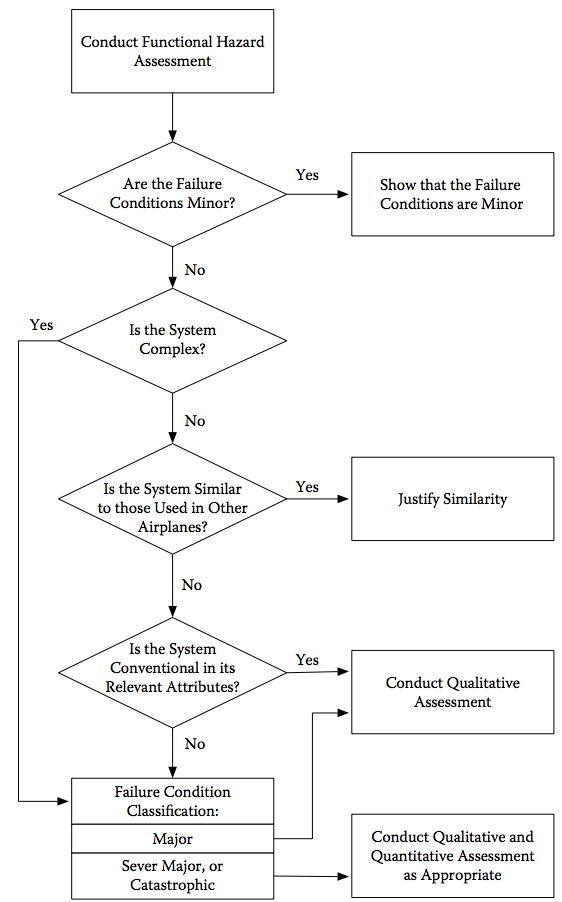
\includegraphics[width=.5\linewidth]{images/complianceFlow.png}
\end{center}

\subsection*{So Many Standards, So Little Time}
\begin{itemize}
    \item research in the past often in single countries
    \item regulations may be there to protect local economy
    \item \emph{common aspects}
    \begin{description}
        \item[prescription level] some documents are compulsory, other recommended (best practices)
        \item[reference sector] different markets, different (safety requirements), different traditions, different engineering practices/ constraints
        \item[Scope] standards for software, hardware, complex systems
    \end{description}
\end{itemize}

\subsection*{The ECSS System of standards}
\begin{itemize}
    \item standards of the european space agency
    \item no legal standing, but covers all aspects of space engineering
    \begin{description}
        \item[M] \emph{space project management branch} management
        \item[Q] \emph{space product assurance} quality assurance, system safety
        \item[E] \emph{space engineering branch} systems engineering, software engineering
        \item[S] \emph{standards}
    \end{description}
\end{itemize}
\begin{center}
    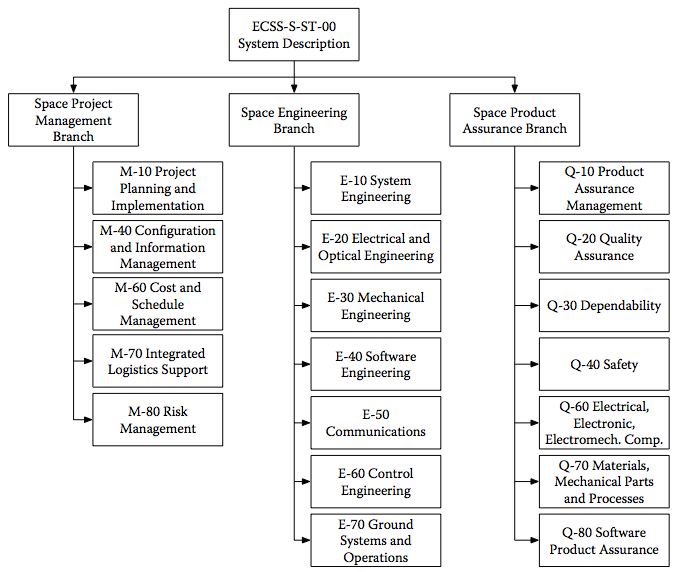
\includegraphics[width=.5\linewidth]{images/ecss.png}
\end{center}

\subsection*{Avionics Reference Standards}
\begin{center}
    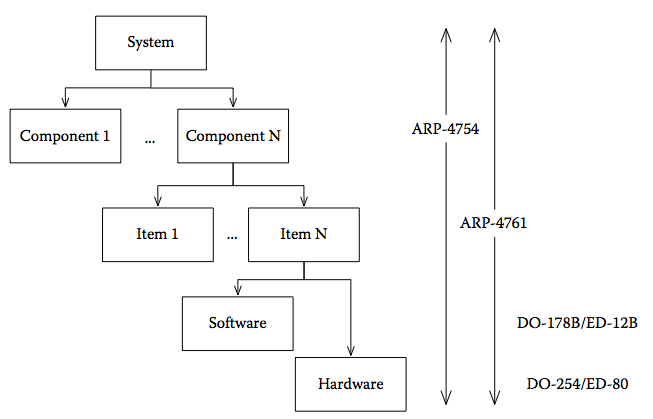
\includegraphics[width=.5\linewidth]{images/arp.png}
\end{center}
\begin{itemize}
    \item standards cover different aspects of system development
    \begin{description}
        \item[Highly-Integrated or Complex Aircraft Systems]
        \item[Safety Asessment on Civil Airborne Systems and Equipment]
        \item[Software Considerations]
        \item[Airborne Electronics Hardware]
    \end{description}
\end{itemize}

\subsection*{ARP 4754}
\begin{itemize}
    \item certification aspects of system that implement aircraft-level functions (e.g. fly-by-wire system)
    \item document focuses on development and certification of complex systems to include
    \begin{description}
        \item[system development] top-down development
        \begin{itemize}
            \item describes how the previously mentioned processes integrate into coherent development process
            \item iterative process, increasing levels of refinement
            \item runs parallel and integrates with safety assessment activities
            \item main development activities:
            \begin{description}
                \item[aircraft-level functional requirements] high-level requirements and functions are defined
                \item[allocation of aircraft functions to systems] functions of previous step are allocated to systems
                \item[development of system architecture] architecture development to implement functions and satisfy safety requirements
                \item[allocation of item requirements to hardware and software]
                \item[system implementation]
            \end{description}
            \item \emph{support processes}
            \begin{itemize}
                \item certification coordination
                \item safety assessment
                \item requirement validation
                \item implementation validation
                \item configuration management
                \item process assurance
            \end{itemize}
        \end{itemize}
        \item[certification process and coordination] methods and techniques to demonstrate compliance of system with certification authorities
        \begin{enumerate}
            \item \emph{certification planning} allows to conciliate development constraints, system complexity and certification activities
            \item \emph{agreement on the proposed means of compliance} allows to accommodate special conditions
            \item \emph{Compliance substantiation} implementation of certification plan
        \end{enumerate}
        \item[requirement determination and assignment of development assurance levels] how allocation of critical safety requirements determines assurance levels of components
        \begin{itemize}
            \item five levels of criticality
            \item techniques for safety improvement
            \begin{description}
                \item[partitioning] isolate critical components \follows lower levels of assurance for non-critical components
                \item[redundancy]
                \item[monitoring] redundancy with hot or cold standby
            \end{description}
            \item redundancy:
            \begin{description}
                \item[similar design] redundant design is based on same physical phenomena and component
                \item[dissimilar independent design] redundant design is based on different physical phenomena and components
                \item[dissimilar dependent design] redundant design based on same physical phenomena, but other components
            \end{description}
            \item redundant design \follows reduced chance for complete failure \follows lower level of assurance for single components (if dissimilar)
            \item human intervention \follows lower level of assurance may be possible
        \end{itemize}
        \item[safety assessment process] overview over activities and techniques
        \begin{itemize}
            \item if assurance level are $A$ to $C$, probability below certain value must be shown
        \end{itemize}
        \item[validation of requirements] process and methods to demonstrate that the requirements are complete and specify the ``right system''
        \begin{description}
            \item[validation planning] methods to demonstrate compliance are determined
            \item[execution of checks] actual validation activities
            \item[validation of assumptions] all assumptions during development are listed and validated
        \end{description}
        \begin{itemize}
            \item traceability is important
        \end{itemize}
        \item[implementation verification] demonstrate, that implementation implements all requirements
        \begin{description}
            \item[inspections and reviews] often based on checklists
            \item[analysis] evidence of compliance through detailed examination
            \item[testing] demonstrate implementation of requirements, maybe demonstrate, that undesired functions are not implemented
            \item[service experience] already certified components are used to their specifications
        \end{description}
        \item[configuration management] describe activities to be performed to ensure coherent documentation
        \item[process assurance] describe activities necessary to ensure that development and support process have been dutifully applied and executed
    \end{description}
\end{itemize}

\subsection*{ARP 4761}
\begin{itemize}
    \item ``Guidelines and Methods for Conducting the Safety Assessment Process on Civil Airborne Systems and Equipment''
    \item \emph{Safety Assessment Process}
    \begin{description}
        \item[Fault Hazard Analysis] (FHA) all failures are classified according to severity, including justification for classification
        \item[Preliminary System Safety Assessment] (PSSA) failures identified in FHA are allocated to design components, defines maximum tolerable failure rate
        \item[System Safety Assessment] (SSA) actual design is evaluated wrt target goals of system analysis, failures found in FHA \follows FTA, FMEA, FMES
        \\ Common Cause Analysis is essential
    \end{description}
    \item \emph{Safety Assessment Analysis Method} techniques, that can be used to support safety assessment
\end{itemize}

\subsection*{DO-178B}
\begin{itemize}
    \item EURICAE WG 12 and RTCA Special Committee 167 (1992) \follows common guidance in development of software systems that satisfy airworthiness
    \item different life cycles possible \follows certification achieved by compliance with set of goals:
    \begin{itemize}
        \item development activity type
        \item software category
        \item control category
    \end{itemize}
    \item three kinds of activities characterize development:
    \begin{description}
        \item[software planning process] organize development and support activities
        \item[development process] build a software product
        \item[integral process] ensure correctness and quality of final system
    \end{description}
    \item \emph{software categorized} into five classes $A$ to $E$ according to effect of malfunction
    \item \emph{control category} $CC1$ and $CC2$ defined through $13$ characteristics, e.g. protection against unauthorized changes, $CC1$ is more stringent
\end{itemize}

\subsubsection*{Goals}
\begin{itemize}
    \item for each goal:
    \begin{description}
        \item[description of goal] in natural language
        \item[applicability] allocate achievement of objective to software categories
        \item[output] artifact obtained by achieving the goal
        \item[control category] $CC1$ or $CC2$
    \end{description}
    \item lot of emphasis on testing
\end{itemize}

\subsubsection*{Verification activities}
\begin{description}
    \item[reviews] on high-level artifacts (requirement/design) using common practices
    \item[analyses] often algorithmic
    \item[testing] requirements-based, number of goals dependent on software level
    \item[coverage] different coverages for different software levels
    \begin{itemize}
        \item statement coverage: $A,B,C$
        \item decision coverage: $A,B$
        \item modified condition/decision coverage: $A$
        \item data and control coupling: $A$
    \end{itemize}
\end{description}

\subsubsection*{Certification Goals}
\begin{enumerate}
    \item \emph{certification basis} (agreement between certification authority and applicant, contains special conditions)
    \item \emph{assessment of the ``Plan for Software Aspects of Certification''} how applicant achieves and demonstrates compliance with regulations
    \item \emph{compliance of software} analyze ``Software Accomplishment Summary''
    \begin{itemize}
        \item overview of system and software, certification considerations
        \item software life cycle, data produced during project
        \item software history (change history, unresolved issues)
    \end{itemize}
\end{enumerate}

\subsubsection*{Role of Tools}
\begin{itemize}
    \item any tool can be used, as long as outputs are verified through other means (e.g. automate a task, but not verification)
    \item under special conditions: tools can be used to demonstrate achievemnt of goal
    \begin{description}
        \item[software development tools] output is part of airborne software
        \item[software verification tools] cannot introduce errors, but might fail to detect them
    \end{description}
\end{itemize}

\subsubsection*{Role of Formal Methods}
\begin{itemize}
    \item specific part in ``alternative methods'' part
\end{itemize}

\subsection*{Safety Case}
\begin{itemize}
    \item approach complementary to demonstrating compliances with norms \follows shows that system can be safely operated
    \item demonstrate actual safety instead of compliance with regulations
    \begin{description}
        \item[safety requirements and objectives] define goals of analysis
        \item[safety evidence] define evidence on which analyses rely
        \item[safety argument] describes and argues, how safety evidence is sufficient to demonstrate achievements of safety objectives
    \end{description}
    \item safety case evolves and is refined during development
    \begin{description}
        \item[preliminary safety case] after system requirements have been defined \follows justify the way in which Software Safety Plan delivers System Requirement Specifications that meet safety requirements
        \item[interim safety case] after specifications, demonstrate, that requirements meets safety specifications
        \item[operational safety case] includes set of evidence, that safety requirements have been met
    \end{description}
\end{itemize}

\subsection*{Formal Methods and Certification}
\begin{itemize}
    \item training, tool robustness, tool qualification \follows have to be addressed
    \item \emph{after the fact} system is built, formal methods are used on final product
    \item \emph{parallel} formal activities performed parallel to development of system
    \item \emph{integrated} formal methods are used to drive system development
    \item
\end{itemize}
\begin{center}
    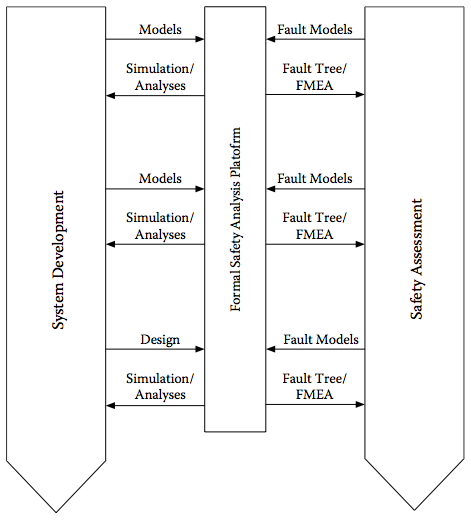
\includegraphics[width=.5\linewidth]{images/safetyDev.png}
\end{center}








678-792

\end{document}
